\documentclass[11pt]{article}
\usepackage{times}
\usepackage[dvips]{graphicx}
\usepackage{latexsym,fullpage,amsmath,listings,graphicx}
%\usepackage{latexsym,fullpage,times}
\usepackage{float,array}
\usepackage[colorlinks]{hyperref}

\newcommand{\onefig}[4]{
\begin{figure}[htb]\hrule
\vspace{3pt}
\begin{center}
\includegraphics[scale=#4]{#1}
\caption{#2} \label{#3}
\end{center}
\vspace{3pt} \hrule
\end{figure}
}

\begin{document}

\begin{center}
{\Large ME/IE/CS 558 -- Spring 2018}\\ \vspace{12pt} {\large
Assignment 3:  Part 1}\\ \vspace{12pt} {\em Due at midnight on March 12, 2018}
\end{center}

{\bf For all assignments:} {\em Unless specifically indicated, you
are free to use any publicly available sources: papers, books,
programs, online material, etc. -- as long as you clearly indicate
and attribute the origin of the information.}

\subsection*{The Task}

In this multi-part assignment, you have to design a program that reads in
$(x,y)$ coordinates of random points and constructs their (otherwise 
unconstrained) Delaunay triangulation and a Voronoi diagram.  
In Part 1 of the assignment, you will design a data structure for the triangulation, 
and will construct an uncosntrained triangulation (not Delaunay) for a given set of points in a plane.  

\subsection*{The Challenge}

The Part 1 of the assignment involves two tasks:  designing a data structure, and 
constructing any valid triangulation.  Specifically:

\begin{itemize}
\item Design a data structure to construct and maintain a
triangulation for a set of points  in the plane. In particular,
your your data structures need to support the following operations
(1) given an edge,
determine the two triangles (faces) sharing it in $O(1)$ time; (2) given a
triangle, determine its vertices (points) and edges in $O(1)$ time; (3) given a
vertex, determine all $k$ edges and triangles sharing it in $O(k)$ time.  The program
must be able to output the list of all edges in the triangulation
(each edge is described by its end points) and the list of all
triangles in the triangulation (each triangle is described by a
triple of points) in $O(n)$ time.

\item Design  an implementable $O(n^2)$ (or better!) algorithm to
construct a triangulation for a set  of points, using one or more
techniques you learned while  studying  algorithms for convex
hulls and polygon triangulation.  Some ideas:  sorting, insertion,
sweeping, divide-and-conquer, etc. (Constructing $O(n^3)$
triangulation is trivial, as we discussed in class. A
triangulation can be also constructed in $O(n \log n)$ time, but
you do not have to produce such an algorithm.)  I encourage you 
to design your own algorithm,  but you  may use
publicly available source code to perform this task, {\em as long
as (1) it does not compute the Delaunay triangulation, and (2) the triangulation is stored in 
your own data structure.}



\end{itemize}

\subsection*{Deliverables}

\begin{description}
\item [Analysis -- 50 points]\hfil\\ For each of the tasks above,
provide all details of your data structures and algorithms
necessary for an implementation.
%Design the crucial tests used in
%constructing a valid triangulation and performing edge flipping.
Estimate the running time of your algorithms, making sure that the
total running time does not exceed $O(n^2)$.


\item[Program -- 50 points] \hfil\\ Implement your data structures
and the algorithm. Assume that  the input file  
{\em testPoints.txt}  contains the list  of test points, each point described by its $x$ and $y$ coordinates:
 $x, y$


Your program will be called from command line as

\begin{lstlisting}

>> python triangle.py filename

\end{lstlisting}

Coordinates file stores n 2D points with the below format.

\begin{lstlisting}

x1 y1
x2 y2
...
xn yn

\end{lstlisting}

Your program should print out the number of triangles, edges, and vertices in the triangulation 
and plot the triangulation (either the edges or the triangles or both) on the screen.
For example, for the following points.txt file

\begin{lstlisting}
0 0
1 0
1 1
0 1
0.5 0.5
\end{lstlisting}

Your program should print the below information.
\begin{lstlisting}
number of triangles = 4
number of edges = 8
number of vertices = 5
\end{lstlisting}
Your program should also plot the triangulation.


\begin{figure}[H]
  \centering
  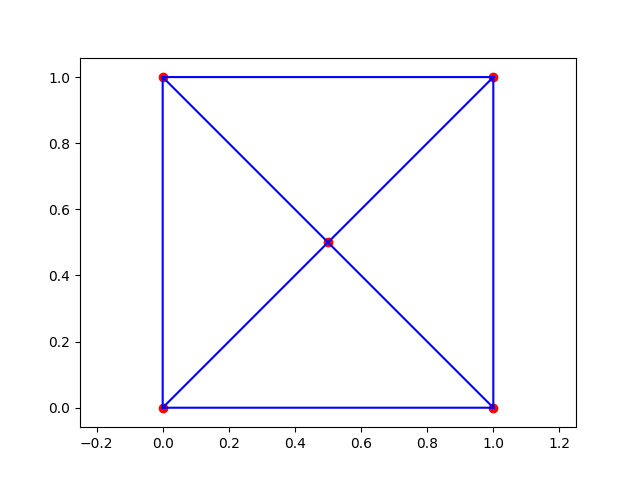
\includegraphics[scale=0.45]{triangle.png}
  \caption{Triangulation example}
  \label{fig:triangle}
\end{figure}


Test your program on a variety of inputs. %, including the test files posted on the course webpage.
Test your program on ability to correctly answer all
other queries mentioned in the assignment. For each test case, print
out the numbers of vertices, edges, and triangles in the constructed
triangulation.   Explain how you chose your tests. 


As usual, the overall structure of your program should be explained and documented; your code should contain appropriate comments.
\end{description}
 
 

\subsection*{Deliverables}

Please use the course website to submit a single  zip  named   FirstName\_LastName\_HW31.zip
The zip archive should contain:  (1) the analysis portion of the assignment,  (2)  the documented python source file, and (3) a PDF readme file  specfying the instructions for running the code.  It should also include at least 1 sample run with input and output,  and specify any specific dependencies or requirements of your code.   

\end{document}


